%!TEX root = Thesis.tex
\chapter{State of the Art}
The following chapter covers an overview and analysis of the existent solutions in
the related research areas of web-based third-party applications, which were designed specially for retrieving differet type of sensed data to the user application. At the beginning the prominent examples of dashboards platforms are studied and evaluated against the requirements described in the previous chapter with a purpose to clarify their individual capabilities.
\section{Frontend Development Approaches}
In computer science, the frontend is responsible for collecting input from user and processing it to a backend system. The frontend is an simply interface between the user and the backend. Therefore, on the one side, generic frontend has to satisfy architecture requirements from backend, such as: fine-grained distributred structure, cross-platforming, multy-user capabilities; and on the other side, define an dynamic user-friendly interface to an end-user.
\newline
To retrieve sensor data from different resources in one web-based interface was created such systems as:
\begin{itemize}
 \item mashup\footnote{\url{http://www.programmableweb.com/applications}},
 \item portal with portlets
 \item HTML5 technology
\end{itemize}
Where the main characteristics of a mashup are combination, visualization and aggregation. Both commercial products and research prototypes have a broad range of features that simplify a mashups design process, and provide mashups storage and publication.
One of the prominent consumer mashup tool is Yahoo Pipes\footnote{\url{http://pipes.yahoo.com/pipes/}}, which allows to create new data mashups via a visual editor by mixing different feed types. Another example is DERI Pipes\footnote{\url{http://pipes.deri.org/}} tool, which is similar to Yahoo Pipes, but enhanced with the possibility to handle the Resource Description Framework (RDF) format. Different from the data pipes Intel Mash Maker\footnote{\url{http://software.intel.com/en-us/articles/intel-mash-maker-mashups-for-the-masses}} is implemented as a web browser’s extension. While browsing a web page, the Mash
Maker toolbar suggests possible additions, e. g. widgets, to the current page, which
extend its capabilities and provide addition information from the other web sites. Mashup composition tools are usually simple enough to be used by end-users for collaborative work. And it fulfill they generally do not require programming skills and rather support visual wiring of GUI widgets, services and components together. On other hand, to customize retrived resources end-user have no option, as using only predefined type and numbers of tools, that was created by system developer.
\newline
Portal technology brings information together from diverse sources in a uniform way. Usually, each information source gets its dedicated area on the page for displaying information (a portlet); often, the user can configure which ones to display. The extent to which content is displayed in a 'uniform way' may depend on the intended user and the intended purpose, as well as the diversity of the content. Very often design emphasis is on a certain 'metaphor' for configuring and customizing the presentation of the content and the chosen implementation framework and/or code libraries\cite{pautasso2008restful,seong2006usability}. In portal technologies end-user can customize number of retrieved data sources, but for that he has to be aware what is it and how to integrate it in portal. User interface in portals have fixed layout, style and location on the web page. To make changes in it, end-user needs to have a deep knowlendge of the system structure and of whole portal entirely.

\section{HTML5 Technology}
HTML5 is based on various design principles, that truly embody a new vision of possibility and practicality\cite{hickson2011html5}.
\begin{itemize}
\item Compatibility(inharit all previous techniques and standards)
\item Utility
\item Secure by Design(origin-based security model that is not only easy to use but is also used consistently by different APIs.)
\item Separation of Presentation and Content(CSS3)
\item Interoperability(Native browser ability instead of complex JavaScript code; a new, simplified DOCTYPE;simplified character set declaration; powerful yet simple HTML5 APIs)
\item Universal Access(suport users with disabilities by using screen readers; media independence-HTML5 functionallity should work across all different devices and platforms; support for all world languages)
\end{itemize}

\section{Sensor Data Retrieval Systems}
 Since the thesis is targeted at the creation of a generic user-friendly data stream interaction system and currently every project focused on a specific area of realization and concrete sensor types, such as urban environment\cite{song2010real}. The real-time environmental monitoring portal or geospatial infrastructure for effectively or
 efficiently collecting and serving vast field data over the web. Internet based urban
environment observation system that can real-time monitor environmental changes of temperature, humidity, illumination or air components in urban area. It provides web-based platform, where end-user can simply monitor urban area in his/her city. In environmental monitoring, the field server for constructing outdoor sensor network is a Web-based field observation device, which detects field environmental parameters and publishes them on Internet in real-time.

 smart city\cite{6588063}tool using information technology and communication (ICT) to help local government to monitoring what currently happened in the city. pplication for monitoring city in single dashboard to help summarize the current condition of city. The architecture system use network sensor consisting of sensor nodes that has
function to capture city condition like temperature, air pollution,
water pollution, traffic situation. Also we can add another information socio-economic situation like public health service, economic indicator, energy supplies, etc. We have successfully developed the prototype of the smart city dashboard the give
more accurate information of Bandung City, one of big cities in Indonesia.
This study has implemented prototype system of smart city dashboard at Bandung. It consists of network sensor, server, application and also communication protocol which is used for
city monitoring. The summary information of city can be displayed in single view to help people watching, analyzing and action to what being happen to city.
 
 LiveWeb\cite{yang2011liveweb}

 robots\cite{bendel2013service}.

Many of the Web applications seen today incorporate different patterns to merge
functionality directed toward the end user. This section focuses on the design approaches for portal solutions. 
It addresses the design stage of the solution development process, highlighting the key issues that are specific to portal and application designs.

\section{Model-View-Control Pattern}
In the design shown in Figure 1 on page X Model represents the application
object that implements the application data and business logic. The View is
responsible for formatting the application results and dynamic page construction.
The Controller is responsible for receiving the client request, invoking the
appropriate business logic, and based on the results, selecting the appropriate
view to be presented to the user.
The Model represents enterprise data and the business rules that govern
access to and updates to this data. Often the Model serves as a software
approximation to a real-world process, so simple real-world modeling
techniques apply when defining the Model.
A View renders the contents of a Model. It accesses enterprise data through
the Model and specifies how that data should be presented.
It is the View's responsibility to maintain consistency in its presentation when
the Model changes. This can be achieved by using a push Model, where the
View registers itself with the Model for change notifications, or a pull Model,
where the View is responsible for calling the Model when it needs to retrieve
the most current data.
A Controller translates interactions with the View into actions to be performed
by the Model. In a stand-alone GUI client, user interactions could be button
clicks or menu selections, whereas in a Web application, they appear as GET
and POST HTTP requests. The actions performed by the Model include
activating business processes or changing the state of the Model. Based on
the user interactions and the outcome of the Model actions, the Controller
responds by selecting an appropriate View.
\begin{figure}[!ht]
\centering
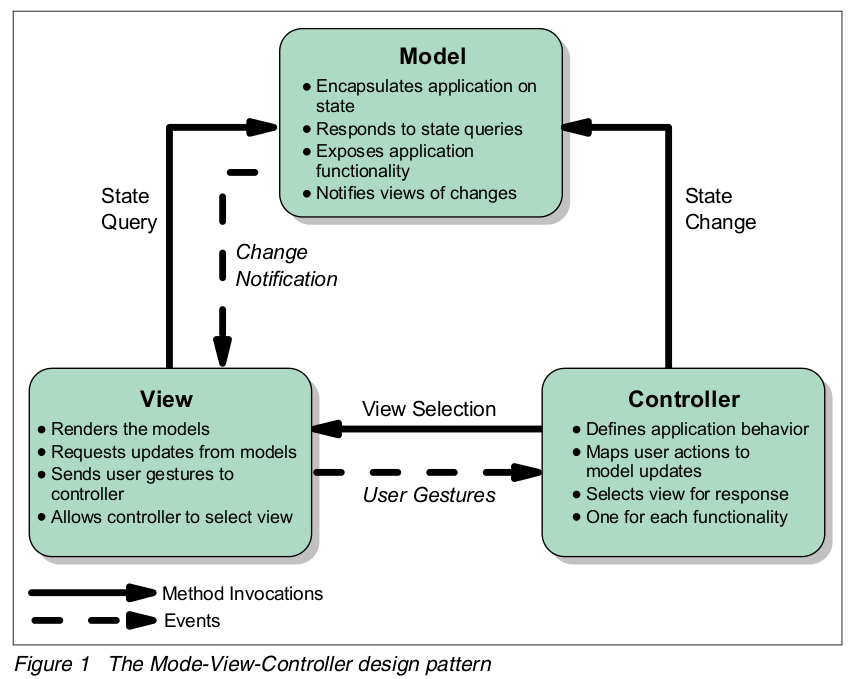
\includegraphics[scale=0.7]{images/MVCPattern.png}   
\caption[MVC Pattern]{MVC Pattern}
\label{img:MVCPattern}                           
\end{figure}
%\footnotetext{Image taken from \url{blog.csdn.net/cain/article/details/6617173}}
\section{Browser Based Collaborative Systems}

\section{Non-Browser Based Collaborative Systems}

\section{Summary}
This chapter briefly introduced main approaches for building web-based dashboards by retriving sensed data. Main focus was given to its multy-user usability, adaptive UI design, dynamic content composition.
